\subsection{Objectifs}

\imgfullw{../img/goal_by_zi3000.jpg}
	{Notre objectif $\cdots$ \hfill $\cdots$ votre objectif}
	{http://zi3000.deviantart.com/art/goal-59036635}

\begin{frame}{Objectifs du cours}
\begin{itemize}
	\item initiation � la programmation 
	\item apprentissage de bons comportements
	\item impl�mentation sur un OS (\textit{operating system})
\end{itemize}
\note[item]{Aborder des th�mes comme : lisibilit�, robustesse, documentation, tests}
\note[item]{Capacit�s de d�vemrinage}
\note[item]{Autonomie dans le travail}
\note[item]{On peut aussi aborder le choix du langage. Pourquoi Java ?}
\end{frame}

\begin{frame}{Liens avec les autres cours}
	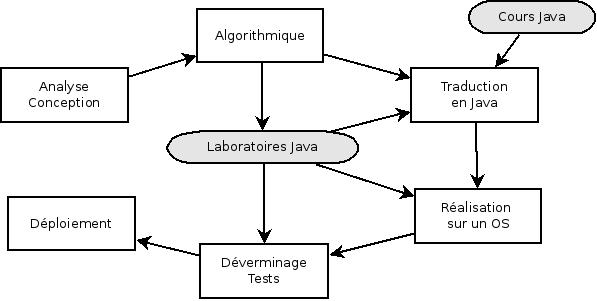
\includegraphics[width=\linewidth]{../img/etapes-SI.jpeg}
\end{frame}

\subsection{Moyens}

\begin{frame}{Supports et ressources}
\emph{Rien} 
\begin{itemize}
  \item pas de syllabus;
  \item pas de livre;
\end{itemize}
\bigskip
\emph{Quoique}
\begin{itemize}
	\item les slides sur \href{https://github.com/HEB-ESI/DEV1-JAV-Slides}{github};
	\item des liens, des documents\dots{} sur \href{https://elearning.esihheb.be}{po�SI} ;
	\item un forum de discussion, \href{http://fora.namok.be}{fora}.
\end{itemize}
\end{frame}

\subsection{�valuations}

\imgfullw{../img/OMG_Spaghetti_O__s_by_billyunderscorebwa.jpg}
	{\centering\huge\color{white}{�valuation � quelle sauce ?}}
	{http://framedbynature.deviantart.com/art/OMG-Spaghetti-O-s-81044629}

\begin{frame}{�valuation}
	�valuation de l'unit� d'enseignement (UE), 
	\\une cote pour toutes les activit�s d'apprentissage (AA):
	\bigskip
	\begin{center}
		{\color{darkgray}\large\bf 
			$\overbrace{\text{ALG - JAV - LAJ}}^{\text{DEV1}}$
		}
	\end{center}
\end{frame}

